% By Fons van der Plas

\documentclass[border=5mm]{standalone}\usepackage{tikz}\usetikzlibrary{calc}\usepackage{amsmath,amssymb}\newcommand{\mat}[1]{\ensuremath{\boldsymbol{\mathrm{#1}}}}\newcommand{\mel}[1]{\ensuremath{{\mathrm{#1}}}}\newcommand{\phym}[1]{\ensuremath{\mathsf{#1}}}\begin{document}

\usetikzlibrary{arrows, decorations.pathmorphing}


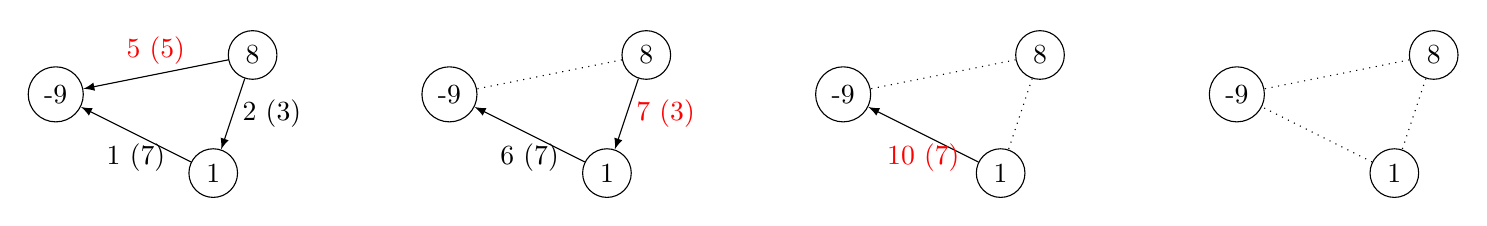
\begin{tikzpicture}[scale=.5]
    \node[draw, circle](b1) at (6,3){8};
    \node[draw, circle](f1) at (1,2){-9};
    \node[draw, circle](l1) at (5,0){1};
    
    
    \draw[-latex] (b1) -- node[midway, right] {2 (3)} (l1);
    \draw[-latex] (l1) -- node[midway, below]{1 (7)} (f1);
    \draw[-latex] (b1) -- node[midway, above]{\color{red}{5 (5)}} (f1);
    
    
    \node[draw, circle](b2) at (16,3){8};
    \node[draw, circle](f2) at (11,2){-9};
    \node[draw, circle](l2) at (15,0){1};
    
    
    \draw[-latex] (b2) -- node[midway, right] {\color{red}{7 (3)}} (l2);
    \draw[-latex] (l2) -- node[midway, below]{6 (7)} (f2);
    \draw[dotted] (b2) --  (f2);
    
    
    \node[draw, circle](b3) at (26,3){8};
    \node[draw, circle](f3) at (21,2){-9};
    \node[draw, circle](l3) at (25,0){1};
    
    
    \draw[dotted] (b3) -- (l3);
    \draw[-latex] (l3) -- node[midway, below]{\color{red}{10 (7)}} (f3);
    \draw[dotted] (b3) --  (f3);
    
    
    \node[draw, circle](b4) at (36,3){8};
    \node[draw, circle](f4) at (31,2){-9};
    \node[draw, circle](l4) at (35,0){1};
    
    
    \draw[dotted] (b4) -- (l4);
    \draw[dotted] (l4) -- (f4);
    \draw[dotted] (b4) --  (f4);
\end{tikzpicture}


\end{document}